\documentclass{article}
\usepackage{fontspec}
\pagestyle{empty}
\usepackage{geometry}
\geometry{paperwidth=100mm, paperheight=100mm, left=2mm, top=0mm, right=2mm, bottom=0mm}
\parindent=0pt
\usepackage{color}
\usepackage{xcolor}
\usepackage{tikz}
\usetikzlibrary{positioning}

\begin{document}
\centering
\vspace*{\fill} \vspace*{-5ex}

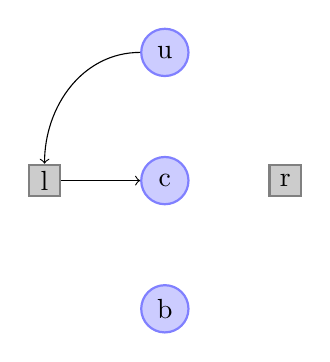
\begin{tikzpicture}[place/.style={circle,draw=blue!50,fill=blue!20,thick,
inner sep=0pt,minimum size=6mm},
transition/.style={rectangle,draw=black!50,fill=black!20,thick,
inner sep=0pt,minimum size=4mm}]
    \node[place] (Node u) {u};
    \node[place] (my center) [below=of Node u] {c};
    \node[place] (Node b) [below=of my center] {b};
    \node[transition] (Node r) [right=of my center] {r};
    \node[transition] (Node l) [left=of my center] {l};
    \draw [->] (Node l) to (my center);
    \draw [->] (Node u) to [out=180,in=90] (Node l);
\end{tikzpicture}
\vspace*{\fill} 
\end{document}